% !TEX program = xelatex
\documentclass{matthijs}

\newcolumntype{R}{>{\arraybackslash}m{10cm}}

% Style for first and last page
\usepackage{wallpaper}
\usepackage{color}
%\definecolor{arobsblue}{HTML}{0e2642}
%\definecolor{arobsblue}{HTML}{0f2c4c}
\definecolor{arobsblue}{HTML}{0e335c}

\usepackage{csquotes}
\usepackage[style=ieee]{biblatex}
\addbibresource{research.bib}

% Versioning
\usepackage[maxdepth=2]{gitinfo2}

% Figures
\usepackage{tikz}
\usepackage{amsmath}

%\usepackage{atbegshi}
%\AtBeginShipout{
%	\begin{tikzpicture}[remember picture,overlay]
%		\fill (current page.north west) node[below right,fill=arobsblue,draw=arobsblue,minimum width=\paperwidth,minimum height=2ex] (box) {};
%	\end{tikzpicture}
%}

\begin{document}

	% Set language to English
	\taal{en}

	% Cover page
	\begin{titelpagina}
		\color{white}

		\titel{\vspace{50pt}Research into Lane Detection Algorithms for FPGAs}{\emph{Project Lane Detection using FPGAs}}
		\author{
			\begin{tabular}{r l}
				\textbf{Author:} & Matthijs Bakker{\color{white}\footnote{\color{white}\textsuperscript{1} s1142121@student.windesheim.nl}} \\
				\textbf{Course:} & HBO-ICT ESA Full-Time \\
				\\
				\textbf{Company:} & AROBS Transilvania SA, Cluj-Napoca, Romania \\
				\textbf{Company Supervisor:} & Pangyu Jeong \\
				\textbf{Windesheim Supervisor:} & Willie Conen \\
				\\
				\textbf{Version:} & 0.1 \\
				\textbf{Commit:} & \gitAbbrevHash @master \\
			\end{tabular}
			\vspace{8ex}
		}

		\ThisULCornerWallPaper{1.001}{asset_bg_first_page.jpg}
		
	\end{titelpagina}

	\pagenumbering{arabic}
	\thispagestyle{empty}

	\begin{hoofdstuk*}{Abstract}

		\textbf{[todo:]}

	\end{hoofdstuk*}

	\begin{inhoudspagina}

	\end{inhoudspagina}

	\pagenumbering{arabic}

	\begin{hoofdstuk}{Introduction}

		A run-off-road crash is a type of accident involving a single vehicle in which it veers off the road and collides with a natural or artificial object \cite{liu2009factors}.
		A study conducted in 2008 by the U.S. Department of Transportation indicated that 45 percent of all fatal highway crashes in the USA that year were run-off-road crashes \cite{dod2011run}.
		For more than 95 percent of these run-off-road crashes, the cause of the crash was attributed to the driver of the vehicle \cite{dod2011run}.
		Another report published by the University of Minnesota shows that the aforementioned number may be as high as 53 percent \cite{edwards2013pilot}.
		In that report, numerous countermeasures were proposed to alert the driver if their car was headed off the road, such as delivering haptic feedback through the steering wheel and giving auditory warnings to the driver.
		However, while countermeasures were proposed, this paper did not clarify when these countermeasures should be triggered or how the car should detect if it is veering off the road.
		
		\bigskip

		To improve the safety of vehicles, AROBS has been developing an Advanced Driver-Assistance System -- hereafter referred to as an ADAS.
		This system comprises of numerous subsystems which monitor and control certain processes inside of the car.
		One of these subsystems is the Lane Departure Warning System \cite{el2020novel}.
		As the name implies, this component of the ADAS assists the driver in keeping the vehicle within in a road lane.
		To detect if the car is properly centered, a camera is positioned on the dashboard of the car and it is faced towards the road.
		The approximate position of the vehicle relative to the road lane is calculated by feeding the video feed from the camera through an algorithm.
		If the result of this process indicates that the car is deterring from the lane, a signal is sent to the ADAS so that a warning can be provided to the driver of the vehicle.
		
		\bigskip

		The goal of this research is to select the best suited algorithm for detecting \textbf{road lane markings} from a video feed and calculating the approximate location of the car relative to the lane.
		It is vital that we spend time on making sure that the selected algorithm fits with the project, because the next phase of the project depends on the information that is gained from this research.

		\bigskip

		This paper is written using the IMRaD format, because it is what we were taught to use at Windesheim.
		However, I realise that this might not be the best format to write the paper in, because the results section is exceptionally big compared to the other sections.
		I have tried to spread out the findings in the results section as much as possible by creating (sub-)sections for different topics.

	\end{hoofdstuk}

	\begin{hoofdstuk}{Methods}

		\begin{paragraaf}{Literature Study}

			First of all, I will set up a literature study to search for existing lane marking algorithms by using various online document aggregators such as Google Scholar and ResearchGate.
			It will be interesting to gauge which algorithms are used in similar projects, because it helps us narrow down on the wide choice of available algorithms.
			Because some papers share common stages in their algorithm, like the usage of the Sobel operator or the Hough transform, I will gather more information on these stages and why they are used in this field.
			It will also be helpful to search if people have made optimizations or variations upon these standard procedures.
			An example of such a variation is an optimized straight-lane Hough Transform targeting FPGAs \cite{el2020novel} which has a higher performance ceiling because it can be parallelized.

		\end{paragraaf}

		\begin{paragraaf}{Test Implementation}

			A trend I have noticed among research on computer vision topics is that researchers first implement the proposed algorithms in MATLAB or a Python script before creating the end product.
			This approach to researching sounds good to me because it gives me a chance to prove that I am not only able to write about these algorithms but that I'm also able to put them to use.
			I'm not yet familiar with the previously mentioned programming languages, so I will use the C language instead.

			\bigskip

			I will implement each of the candidate algorithms in a computer program and run test images through them to determine how effective they are.
			The final chosen algorithm will be implemented on a Field Programmable Gate Array (FPGA), because it needs to be a low-cost device that can analyze the video feed in real-time.
			A selection process will occur, in which the candidate algorithms will be judged by the following metrics:

			\begin{enumerate}

				\item	Accuracy of detection; the effectiveness of the candidate algorithm on test images.
					This metric will be measured by implementing the algorithm into a computer program which can process test images.
					The candidates will be ranked by how accurate the end result is compared to the reference result.

				\item	Environmental suitability; how well the candidate algorithm works when put in different environments.
					This criteria involves using test images that were captured in different weather conditions, lighting conditions and different areas of the world.
					A particular algorithm might work better than others in bright lighting, but may not work at all when the vehicle is driving through a tunnel or at night time.
					The selected test images, as seen in \verwijzing{tabel}{List of test images}, were captured under many different circumstances.
					This metric is measured by the least amount of test images failed to process.

				\item	The feasibility of implementing the candidate algorithm in digital logic.
					It is hard to set up concrete criteria for measuring this metric, because the time and knowledge required to implement a particular algorithm depends on many factors, and it can't be properly calculated in advance.
					For this reason, I will estimate the difficulty of implementing the algorithm in hardware and I will assign it a score between one and five, with five meaning it would be very difficult to implement.

				\item	The resources required to run such an algorithm in real-time.
					We want as little delay as possible between the video frame being shot and the completion of the calculation.
					The quicker the car can detect that it's veering off the lane, the quicker the situation can be rectified, and the safer the system becomes.
					After all, the safety of human lives are at stake.\\
					This metric will be measured by:

					\begin{itemize}

						\item	The average amount of milliseconds it takes for a reference implementation to process one frame
						
						\item	The amount of Look-Up Tables, Flip-Flops and Block RAM a reference implementation occupies

					\end{itemize}

			\end{enumerate}

			The algorithm which scores the best overall on these metrics will be selected to be implemented in digital logic in the next phase of the project.
		\end{paragraaf}

		\begin{paragraaf}{Sample Data Tests}

			To prove the effectiveness of each algorithm, it must be implemented in a computer program which runs a set of test images through it.
			The test images were hand selected from the Berkeley DeepDrive 100K Dataset \cite{yu2020bdd100k} and converted to PPM format for easier manipulation.
			A list of these images, along with the motivation behind why they were selected, can be found in \verwijzing{tabel}{List of test images}.

			\begin{tabel}{List of test images}{l @{\extracolsep{\fill}} R}
				
				\emph{Image Name} & \emph{Motivation} \tabularnewline
				\midrule
				0a0a0b1a-7c39d841.jpg & Clearly defined lane markings, with high contrast between the sky and the road \tabularnewline
				0b16507a-49b0aca9.jpg & Yellow lane marking, to test if the algorithm can detect multiple colors \tabularnewline
				0cf398b3-ce65ab54.jpg & Unclear, partially wiped-out lane markings. This image tests if the algorithm would work in night time as well \tabularnewline
				0d4268d5-3c617dd8.jpg & Off-center vehicle. It would be interesting whether the algorithm detects the left or the right lane \tabularnewline
				0d62200b-85aeaa3d.jpg & Unusual markings on the left side of the lane, not a clear separation between road and curb \tabularnewline
				0fc0b0cc-75d5e23d.jpg & Bad lighting; sunflare disrupts the luminance of the road in the image \tabularnewline
			
			\end{tabel}

		\end{paragraaf}

	\end{hoofdstuk}

	\begin{hoofdstuk}{Results}

		The methods used in the papers that were analyzed shared a common theme: first, the input video feed would be preprocessed and cleaned from artifacts, before being ran through a feature extraction technique like the Hough Transform, and finally being subjected to a line classification technique.
		This preprocessing stage is of high importance, because it directly affects the effectiveness of the feature extraction phase.
		If the features of the image are not properly highlighted, the level of detail remains too high and the feature extraction technique might pick up photographic artifacts as lines.\textbf{[todo: find source]}

		\begin{paragraaf}{Image Preprocessing Techniques}

			According to Malmir et al. \cite{malmir2019design} the main source of difficulty for lane detection is the variation of operating conditions in captured road images.
			An example of this is the variation in colors of the paint used for drawing road markings.
			White paint is common in Europe while yellow paint can be seen in North America.
			The yellow gloom of the sunset can make it harder to detect yellow lane markings on a video frame because they blend in with the environment \cite{tumasov2021research}.
			Though, the use of white paint has a disadvantage as well: pools of water can reflect sunlight and appear as white lane markings \cite{krine2021road}.
			To generify our product and make it work in many different environments, we need to take into account such environmental factors.
			The video feed needs to be preprocessed in such a way that as little artifacts as possible get fed into the Hough transform.
			This decreases the chance that anomalies appear in the result of the Hough transform.
			
			\begin{subparagraaf}{Grayscale Conversion}

				\textbf{[todo:]}
			
			\end{subparagraaf}

			\begin{subparagraaf}{Region of Interest Definition}

				To reduce the computing resources needed to run the algorithm, regions of interest (ROIs) may be defined around where the left and right lane markings are supposed to be \cite{el2020novel}.
				The pixels outside of the defined ROIs will not be processed by the algorithm.
				
				\bigskip

				It can be assumed that the upper portion of a video frame captured by the dashboard camera is above the horizon, meaning that it is not worth scanning for road lanes.
				Thus, it can be safely ignored to save computing resources.

			\end{subparagraaf}

			\begin{subparagraaf}{Noise Reduction}

				\textbf{[todo:]}

				\begin{subsubparagraaf}{Average Filter}

					\textbf{[todo:]}
				
				\end{subsubparagraaf}

				\begin{subsubparagraaf}{Gaussian Filter}

					To smooth the image and prevent false detection of edges, a Gaussian blur is applied to the image.

					\bigskip

					\textbf{[todo:]}

					\textbf{[todo: how is kernel calculated?]}

					\textbf{[todo: kernel in scaled brackets (https://latex-tutorial.com/tutorials/amsmath/)]}

					\textbf{[todo: how is kernel convoluted with the image?]}

					\bigskip

					To determine the value of a pixel, the Gaussian kernel must have information on the neighboring pixels.
					Because the pixels at the edge of the image don't have neighboring pixels (assuming the kernel size is larger than one) they get cut off.
					This explains why the resolution of the output image is smaller than that of the input image.
					\verwijzing{figuur}{Formulae for calculating the dimensions of the result image} suggests how to calculate the width and height of the resulting image based on the resolution of the initial image and the size of the Gaussian kernel.
					In these formulae, $w$ is the width of an image and $h$ is the height of an image.
					Symbols $x$ and $y$ represent the width and height of the Gaussian kernel.

					\begin{figuur}{Formulae for calculating the dimensions of the result image}
						\begin{equation*}
							w_{out} = w_{in} - 2 * (\lfloor(x - 1) / 2\rfloor + 1)
						\end{equation*}

						\vspace{-4ex}
					
						\begin{equation*}
							h_{out} = h_{in} - 2 * (\lfloor(y - 1) / 2\rfloor + 1)
						\end{equation*}
					\end{figuur}

					\begin{figuur}{Example of an image blurred by a Gaussian function}

						\begin{tabular}{ccc}
							
							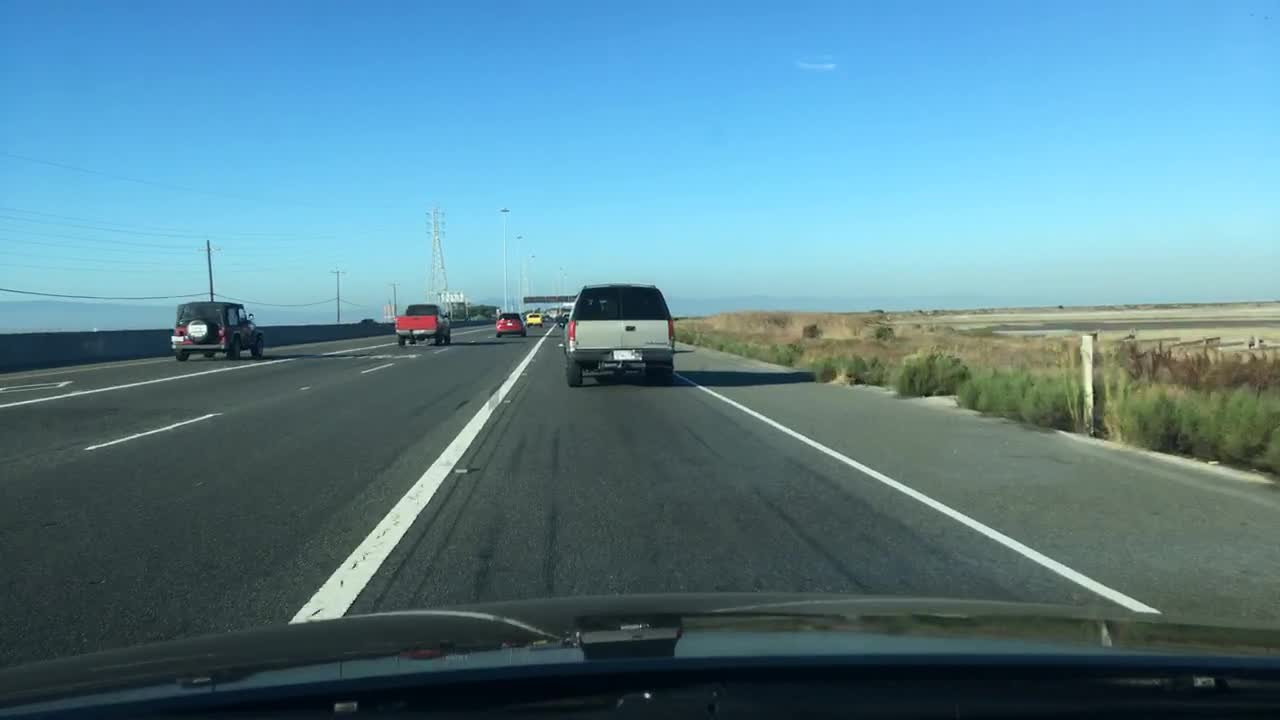
\includegraphics[width=0.3\textwidth]{0a0a0b1a-7c39d841.png} &
							
							\begin{tikzpicture}
								\draw[-to, white](0,0) -- (1,0);
								\draw[-to, thick](0,1.2) -- (1,1.2);
							\end{tikzpicture} &
							
							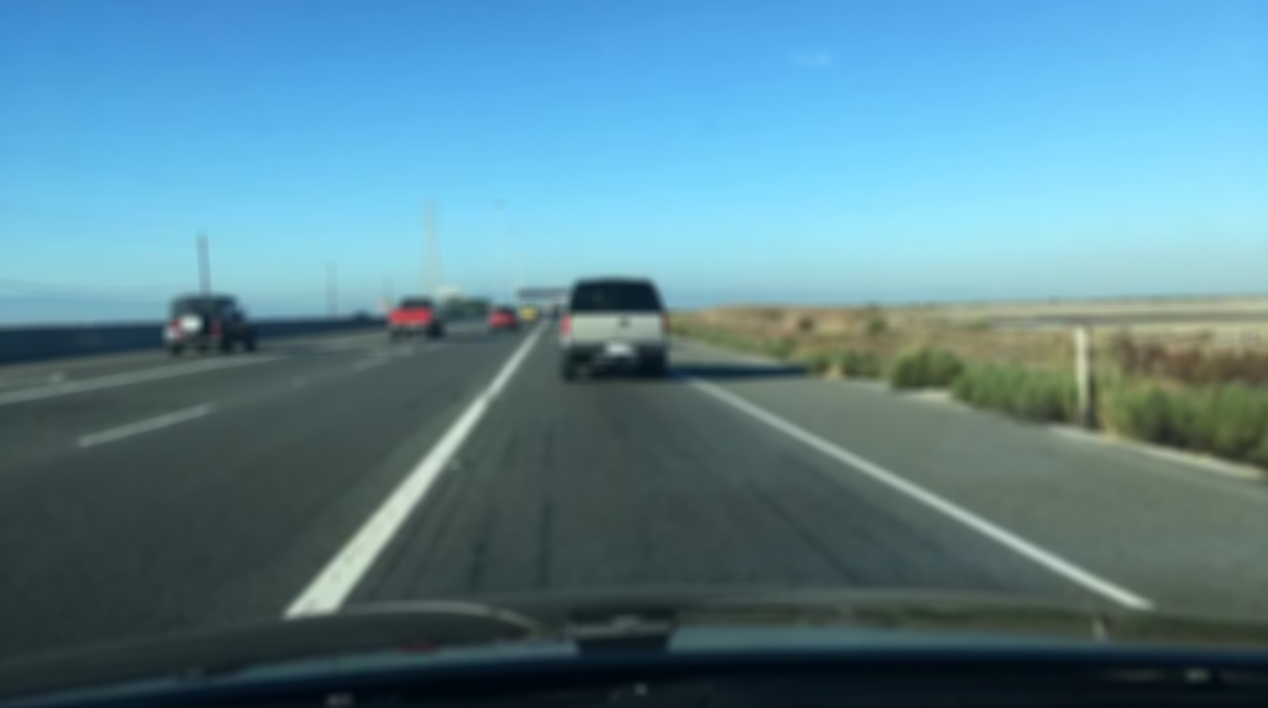
\includegraphics[width=0.3\textwidth]{0a0a0b1a-7c39d841.gaussian.out.png} \\

							&& $ x = y = 10 $ \\
							&& $ \sigma = 6,0 $
							
						\end{tabular}

					\end{figuur}

				\end{subsubparagraaf}

			\end{subparagraaf}

			\begin{subparagraaf}{Edge Detection}

				\textbf{[todo:]}

				\begin{subsubparagraaf}{Sobel-Feldman Operator}

					\textbf{[todo:]}

				\end{subsubparagraaf}

				\begin{subsubparagraaf}{Canny Edge Detector}

					This edge detection technique is not an operator in itself; it suggests a routine around an existing edge detection operator such as the Sobel-Feldman operator.
					\textbf{[todo:]}

				\end{subsubparagraaf}

			\end{subparagraaf}

			\begin{subparagraaf}{Thresholding}

				\textbf{[todo:]}

			\end{subparagraaf}

		\end{paragraaf}

		\begin{paragraaf}{Feature Extraction Techniques}

			\textbf{[todo:]}

			\begin{subparagraaf}{Hough Transform}

				\begin{subsubparagraaf}{Vanishing Point-Based Optimizations}

					\textbf{[todo:]}

				\end{subsubparagraaf}

			\end{subparagraaf}

			\begin{subparagraaf}{Radon Transform}

				\textbf{[todo:]}

			\end{subparagraaf}
		\end{paragraaf}

		\begin{paragraaf}{Line Classification Techniques}

			The resulting data from the Hough transform does not bear any meaning on its own.
			It consists of a set of lines that can represent anything; from actual road markings to cracks in the road and even anomalies in the roadside.
			The goal of the classification part of the algorithm is to detect which lines are the left and right lane markings.

			\begin{subparagraaf}{K-Means Clustering of HT Results}

				The Hough Transform used in the feature extraction phase gives us the extremes of the lane marking lines \cite{gupta2016automated}.
				To convert this into usable data, it must be clustered and grouped into line segments.

			\end{subparagraaf}

			\begin{subparagraaf}{Stripe Detection}

				According to Malmir et al. \cite{malmir2019design}, the Hough transform stage achieves acceptable results 80 percent of the time.
				They suggested that this number decreases during non-ideal conditions such as poor visibility and driving at night time.
				In their work, they proposed a processing stage that occurs after an iteration of the Hough transform and provides reference data for the next iteration.

				\bigskip

				The basic premise of stripe detection is that the difference between video frames is not substantial because they are captured at a high rate.
				Therefore, we may use the stored coordinates of the detected lines in the previous frame as a reference while processing the current frame \cite{malmir2019design}.
				If the difference between the position of the lines in the previous frame and the current frame is within a predefined threshold, we can assume that are the same.
				Else, we distribute candidate points -- so-called 'particles' -- around the position of the line from the previous frame.
				Each particle has a rectangular search area around it.
				In this search area, a convolutional directional edge detection filter is applied to magnify the image features.
				Two kernels are used to find the left- and right edges of the lane marking.
				Once these edges are found, an additional test makes sure that the average brightness of the pixels between the edges on the grayscale image is brighter than that of the surrounding pixels.
				The position of the lane marking is found by stringing together the valid particles.

				\bigskip

				As mentioned in the paper, the effectiveness of this algorithm is highly dependent on the integrity of the result of the Hough transform that is carried out on the first frame of the video feed.
				This is because the algorithm bases its conception of correctness on previous frames of the video.
				The authors tried to overcome this issue by processing the video feed with a stricter threshold until a valid lane marking is found \cite{malmir2019design}.

			\end{subparagraaf}

		\end{paragraaf}

		\begin{paragraaf}{Comparison of Candidate Algorithms}

			\textbf{[todo:]}

		\end{paragraaf}

	\end{hoofdstuk}

	\begin{hoofdstuk}{Conclusion}

		\textbf{[todo:]}

	\end{hoofdstuk}

	\begin{hoofdstuk}{Discussion}

		\textbf{[todo:]}

	\end{hoofdstuk}

	% Bibliography page
	\begin{hoofdstuk}{References}

		\printbibliography[heading=none]
	
	\end{hoofdstuk}

	% Empty last page
	\clearpage
	\thispagestyle{empty}
	\addtocounter{page}{-1}
	\ThisULCornerWallPaper{1.005}{asset_bg_last_page.jpg}
	\
	\clearpage

\end{document}
